%\chapter*{Неделя 9}
\protect\thispagestyle{fancy}
\section{}
Пусть $\Capit{Z}$-преобразование (двухстороннее) дискретного сигнала $x[k]$ имеет вид $\Capit{X}(z) = (z^2 + 2z + 1)/z$.

Найти ненулевые отсчётные значения этого сигнала. Определить, является ли такой сигнал казуальным. 

\begin{align*}
	&\Capit{X}(z) = (z^2 + 2z + 1)/z = z + 2 + z^{-1} = x[-1]z + x[0] + x[1]z^{-1} =  \sum \limits_{-\infty}^{+\infty} x[k]z^{-k},\\
	&x[1] = x[-1] = 1,\quad x[0] = 2.
\end{align*}

При этом $x[-1] = 1 \neq 0$, то есть сигнал не является каузальным.


\section{}
Найти импульсную характеристику $h[k]$ фильтра с передаточной функцией

\begin{equation*}
	\Capit{H}(z) = \dfrac{1 - z^{-1}}{1 + 0.5z^{-1}}
\end{equation*}

\begin{enumerate}
	\item вычислением обратного $\Capit{Z}$-преобразования;
	\item реакцией на единичный импульс $\mathbf{1}[k]$ при начальном условии $y[-1]=0$.
\end{enumerate}

Сравнить результаты. Исследовать фильтр на устойчивость.

Методом геометрических построений определить значения АЧХ и ФЧХ фильтра в точке $\nu_0 = \frac{1}{4}$.

\begin{align*}
	\Capit{H}(z) = \dfrac{1 - z^{-1}}{1 + 0.5z^{-1}} = \dfrac{1}{1 + 0.5z^{-1}} - \dfrac{z^{-1}}{1 + 0.5z^{-1}} \xlongleftrightarrow{\Capit{Z}} h[k] =&\left(-\dfrac{1}{2}\right)^k \s{u}[k] -  \left(-\dfrac{1}{2}\right)^{k-1} \s{u}[k-1] = \\
	=&\left(-\dfrac{1}{2}\right)^k \left(\s{u}[k] + 2 \s{u}[k-1] \right),\quad\text{ROC} = \{z: |z| > 0.5\}.
\end{align*}

\begin{align*}
	x[k] = \mathbf{1}[k] \xlongleftrightarrow{\Capit{Z}} \Capit{X}(z) = 1,
	\quad \Capit{Y}(z) = \Capit{X}(z)\cdot \Capit{H}(z) = \Capit{H}(z) \xlongleftrightarrow{\Capit{Z}} y[k] = h[k] = \left(-\dfrac{1}{2}\right)^k \left(\s{u}[k] + 2 \s{u}[k-1] \right),\\
	\quad\text{ROC} = \{z: |z| > 0.5\}.
\end{align*}

\begin{align*}
	\Capit{H}(z) = \dfrac{1 - z^{-1}}{1 + 0.5z^{-1}} = \dfrac{z - 1}{z + 0.5},\quad
	\Rightarrow z_{\times} = -0.5, z_{o} = 1. 
\end{align*}

\begin{minipage}{0.4\textwidth}
	%\begin{figure}[!h]
	\centering
	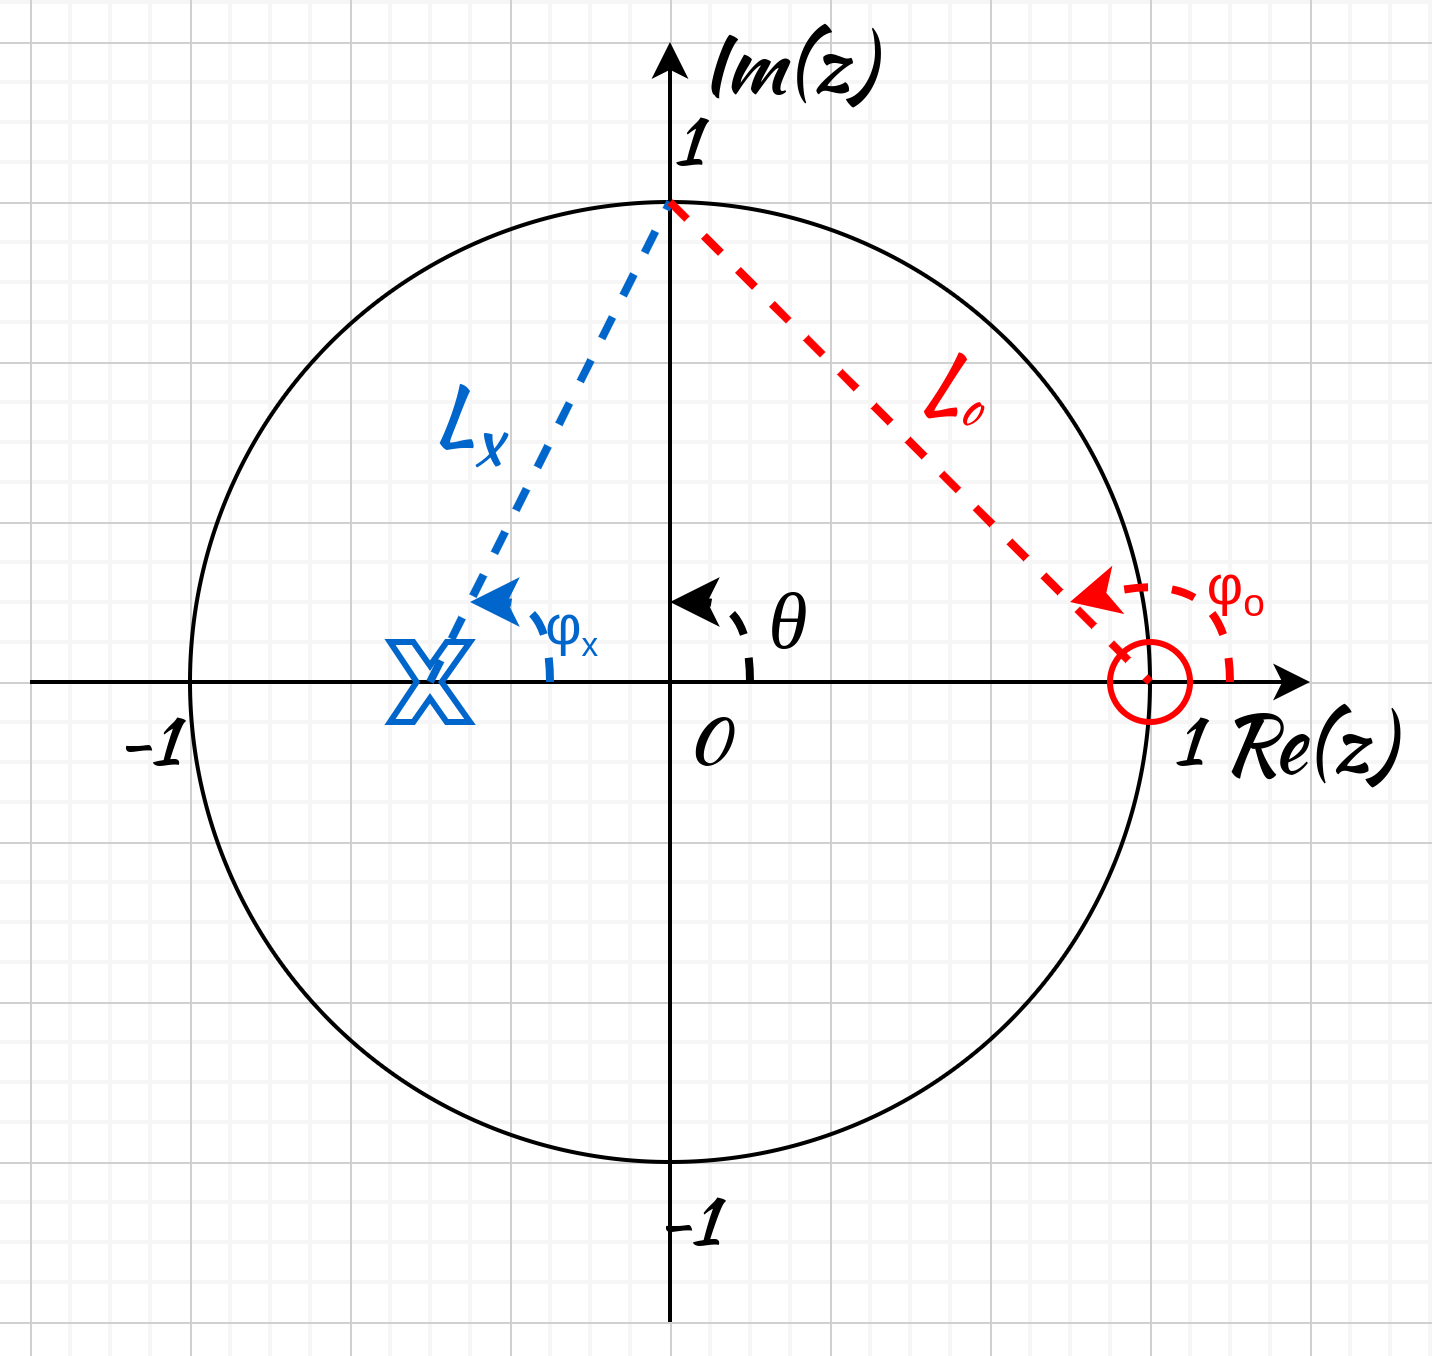
\includegraphics[width=1.\columnwidth]{pics/fall/9/complexplane.png}
	\label{fig:9-2}
	%\end{figure}
\end{minipage}
\hfill
\begin{minipage}{0.4\textwidth}
	\begin{align*}
		&\theta = 2\pi \nu_0 = 2\pi \dfrac{1}{4} = \dfrac{\pi}{2}.\\
		&\varphi(\nu_0) = \varphi(\theta) = \varphi_{o} - \varphi_{\times} = \dfrac{3\pi}{4} - \arctg(2) = 1.249 = 0.397\pi.\\
		&|\Capit{H}(\nu_0)| = |\Capit{H}(\theta)| = \dfrac{L_{o}}{L_{\times}} = \dfrac{\sqrt2}{\sqrt{1 + (0.5)^2}} = \sqrt{\dfrac{8}{5}} = 1.265.
	\end{align*}
\end{minipage}


Единственный полюс $z_{\times} = -0.5$ лежит внутри единичного круга на комплексной плоскости, то есть система является устойчивой по входу.



\section{}
Рассмотрите рекурсивный фильтр, заданный разностным уравнением

\begin{equation*}
	y[k] = (1 - \lambda)x[k] + \lambda y[k-1],\quad y[-1] = 0.
\end{equation*}

При $\lambda \approx 1$, $\lambda < 1$ эта система является квазиинтегратором (leaky integrator).
Определите импульсную характеристику этой системы и исследуйте систему на устойчивость для случаев $\lambda_1 = 1$ и $\lambda_2=0.9$.
Постройте блок-схему для реализации данной системы.

\begin{align*}
	&(1 - \lambda) x[k] = y[k] - \lambda y[k-1],\quad y[-1] = 0.\\
	&\Capit{H}(z) = \dfrac{\Capit{Y}(z)}{\Capit{X}(z)} = \dfrac{1 - \lambda}{1 - \lambda z^{-1}} =
	\dfrac{(1 - \lambda)z}{z - \lambda}  
	\xlongleftrightarrow{\Capit{Z}} h[k] = (1-\lambda)\lambda^k \s{u}[k],\quad\text{ROC} = \{z: |z| > \lambda\}.
\end{align*}

При $\lambda_1=1$ единственный полюс $z_{\times} = \lambda_1 = 1$ находится на границе единичного круга комплексной плоскости, а не внутри него. Значит, система не является устойчивой по входу.


В случае $\lambda_1=0.9$ полюс $z_{\times} = \lambda_1 = 0.9$ находится внутри единичного круга, то есть система будет устойчивой по входу.

\begin{figure}[!h]
	\centering
	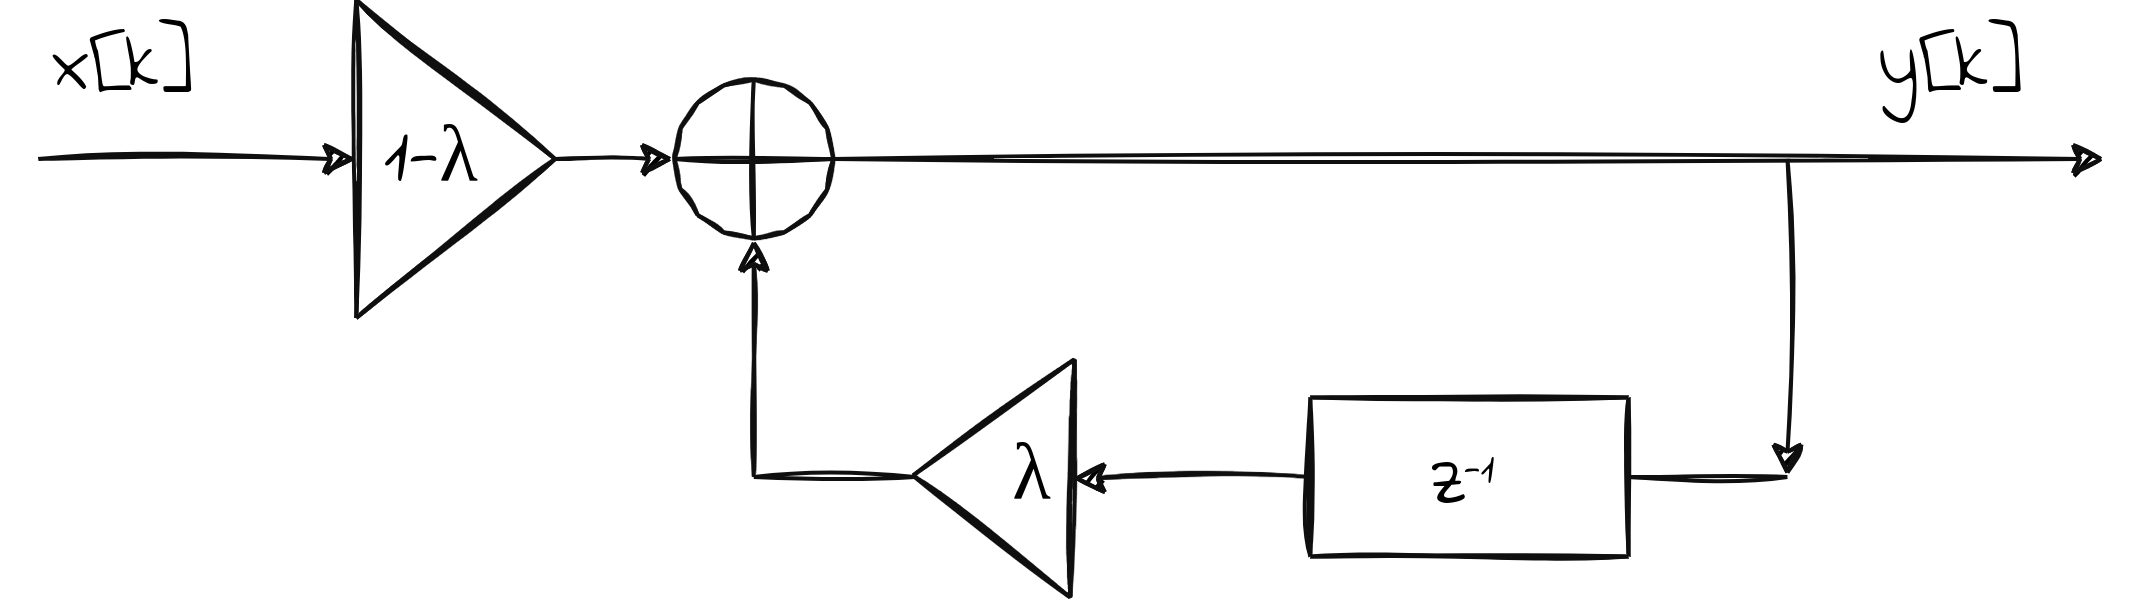
\includegraphics[width=0.8\columnwidth]{pics/fall/9/integrator.png}
	\label{fig:9-3}
\end{figure}

